\chapter{Results}

\section{Cohort of patients}

% TLCR
% Patients were followed from their diagnosis of stage IV disease.

% CCLM
% A total of 54 samples were obtained from 52 NSCLC patients and two healthy donors, after signing the appropriate informed consent.

% TESIS estela
% Para establecer la mejor estrategia metodológica, para la identificación del paciente candidato a recibir un inhibidor de ALK, se emplearán 20 muestras pre-tratamiento, pareadas de plasma y plaquetas, de pacientes con cáncer de pulmón no microcítico con enfermedad avanzada y translocación de ALK documentada según los protocolos asistenciales. Estas muestras se encuentran disponibles en el Biobanco del Hospital Universitario Puerta de Hierro.
% A fin de evaluar la utilidad de la biopsia líquida para monitorizar al paciente con translocación de ALK se reclutarán 30 pacientes, a razón de 15 pacientes por año. De cada paciente se recogerán muestras a los 2, 4, 6, 8, 12, 15 y 18 meses de tratamiento y a la progresión.
% % Los datos demográficos, clínico-patológicos, el estado mutacional del tumor, así como el estado funcional de los pacientes fueron obtenidos de los informes médicos. El ajuste de dosis y el cambio de medicación fueron documentados a lo largo del estudio.
%VARIABLES
% -Progresión de la enfermedad según criterios RECIST.
% -Supervivencia libre de progresión desde el inicio del tratamiento.
% -Supervivencia global desde el inicio del tratamiento.
% -Tasa de respuesta obtenida
% -Status EML4-ALK (positivo o negativo) en la biopsia líquida.
% -Niveles plasmáticos de EML4-ALK

% ALK paper
% In total, 33 plasma and 2 cerebrospinal fluid (CSF) specimens were collected and analyzed. Samples were collected at the time of disease progression which was assessed according to RECIST criteria v.1.


\begin{table}[ht]
\centering
\resizebox{0.65\textwidth}{!}{
\renewcommand{\arraystretch}{1.25}
\begin{tabular}{cccc}
\rowcolor[HTML]{C0C0C0} 
\textbf{Clinical feature} & \textbf{Categorization}  & \textbf{N} & \textbf{\%} \\
\rowcolor[HTML]{FFFFFF}
\textbf{Age of diagnosis} & Median & 54 & \\
\rowcolor[HTML]{EFEFEF}
\cellcolor[HTML]{EFEFEF} & Female & 17 & 56.7\% \\
\rowcolor[HTML]{EFEFEF}
\multirow{-2}{*}{\cellcolor[HTML]{EFEFEF}\textbf{Sex}} & Male & 13 & 43.3\% \\
\rowcolor[HTML]{FFFFFF}
\cellcolor[HTML]{FFFFFF} & Never smokers & 18 & 60\% \\
\rowcolor[HTML]{FFFFFF}
\cellcolor[HTML]{FFFFFF} & Ex-smokers & 8 & 26.7\% \\
\rowcolor[HTML]{FFFFFF}
\multirow{-3}{*}{\cellcolor[HTML]{FFFFFF}\textbf{Smoking status}} & Current smokers & 4 & 13.3\% \\
\rowcolor[HTML]{EFEFEF}
\cellcolor[HTML]{EFEFEF} & 0 & 14 & 46.7\% \\
\rowcolor[HTML]{EFEFEF}
\cellcolor[HTML]{EFEFEF} & 1 & 13 & 43.3\% \\
\rowcolor[HTML]{EFEFEF}
\multirow{-3}{*}{\cellcolor[HTML]{EFEFEF}\textbf{\begin{tabular}[c]{@{}c@{}}ECOG\\ performance status\end{tabular}}} & 2 & 3 & 10\% \\
\rowcolor[HTML]{FFFFFF}
\cellcolor[HTML]{FFFFFF} & Adenocarcinoma & 28 & 93.3\% \\
\rowcolor[HTML]{FFFFFF}
\multirow{-2}{*}{\cellcolor[HTML]{FFFFFF}\textbf{Histology}} & Neuroendocrine carcinoma & 2 & 6.7\% \\
\rowcolor[HTML]{EFEFEF} 
\cellcolor[HTML]{EFEFEF} & IV & 23 & 76.7\% \\
\rowcolor[HTML]{EFEFEF}
\cellcolor[HTML]{EFEFEF} & III & 6 & 20\% \\
\rowcolor[HTML]{EFEFEF}
\multirow{-3}{*}{\cellcolor[HTML]{EFEFEF}\textbf{\begin{tabular}[c]{@{}c@{}}Initial\\ clinical stage\end{tabular}}}  & II & 1 & 3.3\% \\
\rowcolor[HTML]{FFFFFF}
\cellcolor[HTML]{FFFFFF} & Alectinib & 11 & 36.7\% \\
\rowcolor[HTML]{FFFFFF}
\cellcolor[HTML]{FFFFFF} & Crizotinib & 10 & 33.3\% \\
\rowcolor[HTML]{FFFFFF}
\cellcolor[HTML]{FFFFFF} & Ceritinib & 4 & 13.3\% \\
\rowcolor[HTML]{FFFFFF}
\cellcolor[HTML]{FFFFFF} & No treatment & 2 & 6.7\% \\
\rowcolor[HTML]{FFFFFF}
\cellcolor[HTML]{FFFFFF} & Brigatinib & 1 & 3.3\% \\
\rowcolor[HTML]{FFFFFF}
\cellcolor[HTML]{FFFFFF} & Lorlatinib & 1 & 3.3\% \\
\rowcolor[HTML]{FFFFFF}
\multirow{-7}{*}{\cellcolor[HTML]{FFFFFF}\textbf{Treatment}} & Chemotherapy & 1 & 3.3\%
\end{tabular}}
\caption{aaaaaaaa.}
\label{tab:Patients}
\end{table}

\section{Next Generation Sequencing Characterization}

% Todos estos resultados fueron utilizados posteriormente para establecer los parámetros del algoritmo implementado.

\section{Implemented Pipeline}

The development of the bioinformatic pipeline was divided into two steps: the implementation of the filtering algorithm itself; and that of a graphical interface to simplify the process of selecting parameters and saving the output variants along with their properties in a \textit{.csv} file.

\subsection{Algorithm Characterization}

In order to detect all variants at the ALK gene locus, specific conditions for each of them have been established from a set of previously validated samples. The flowchart in \autoref{fig:Algorithm} shows the basic structure of the developed pipeline and the selection criteria based on certain variables as presented in the \textit{non-filtered-oncomine.tsv} file.

\begin{figure}[ht]
    \centering
    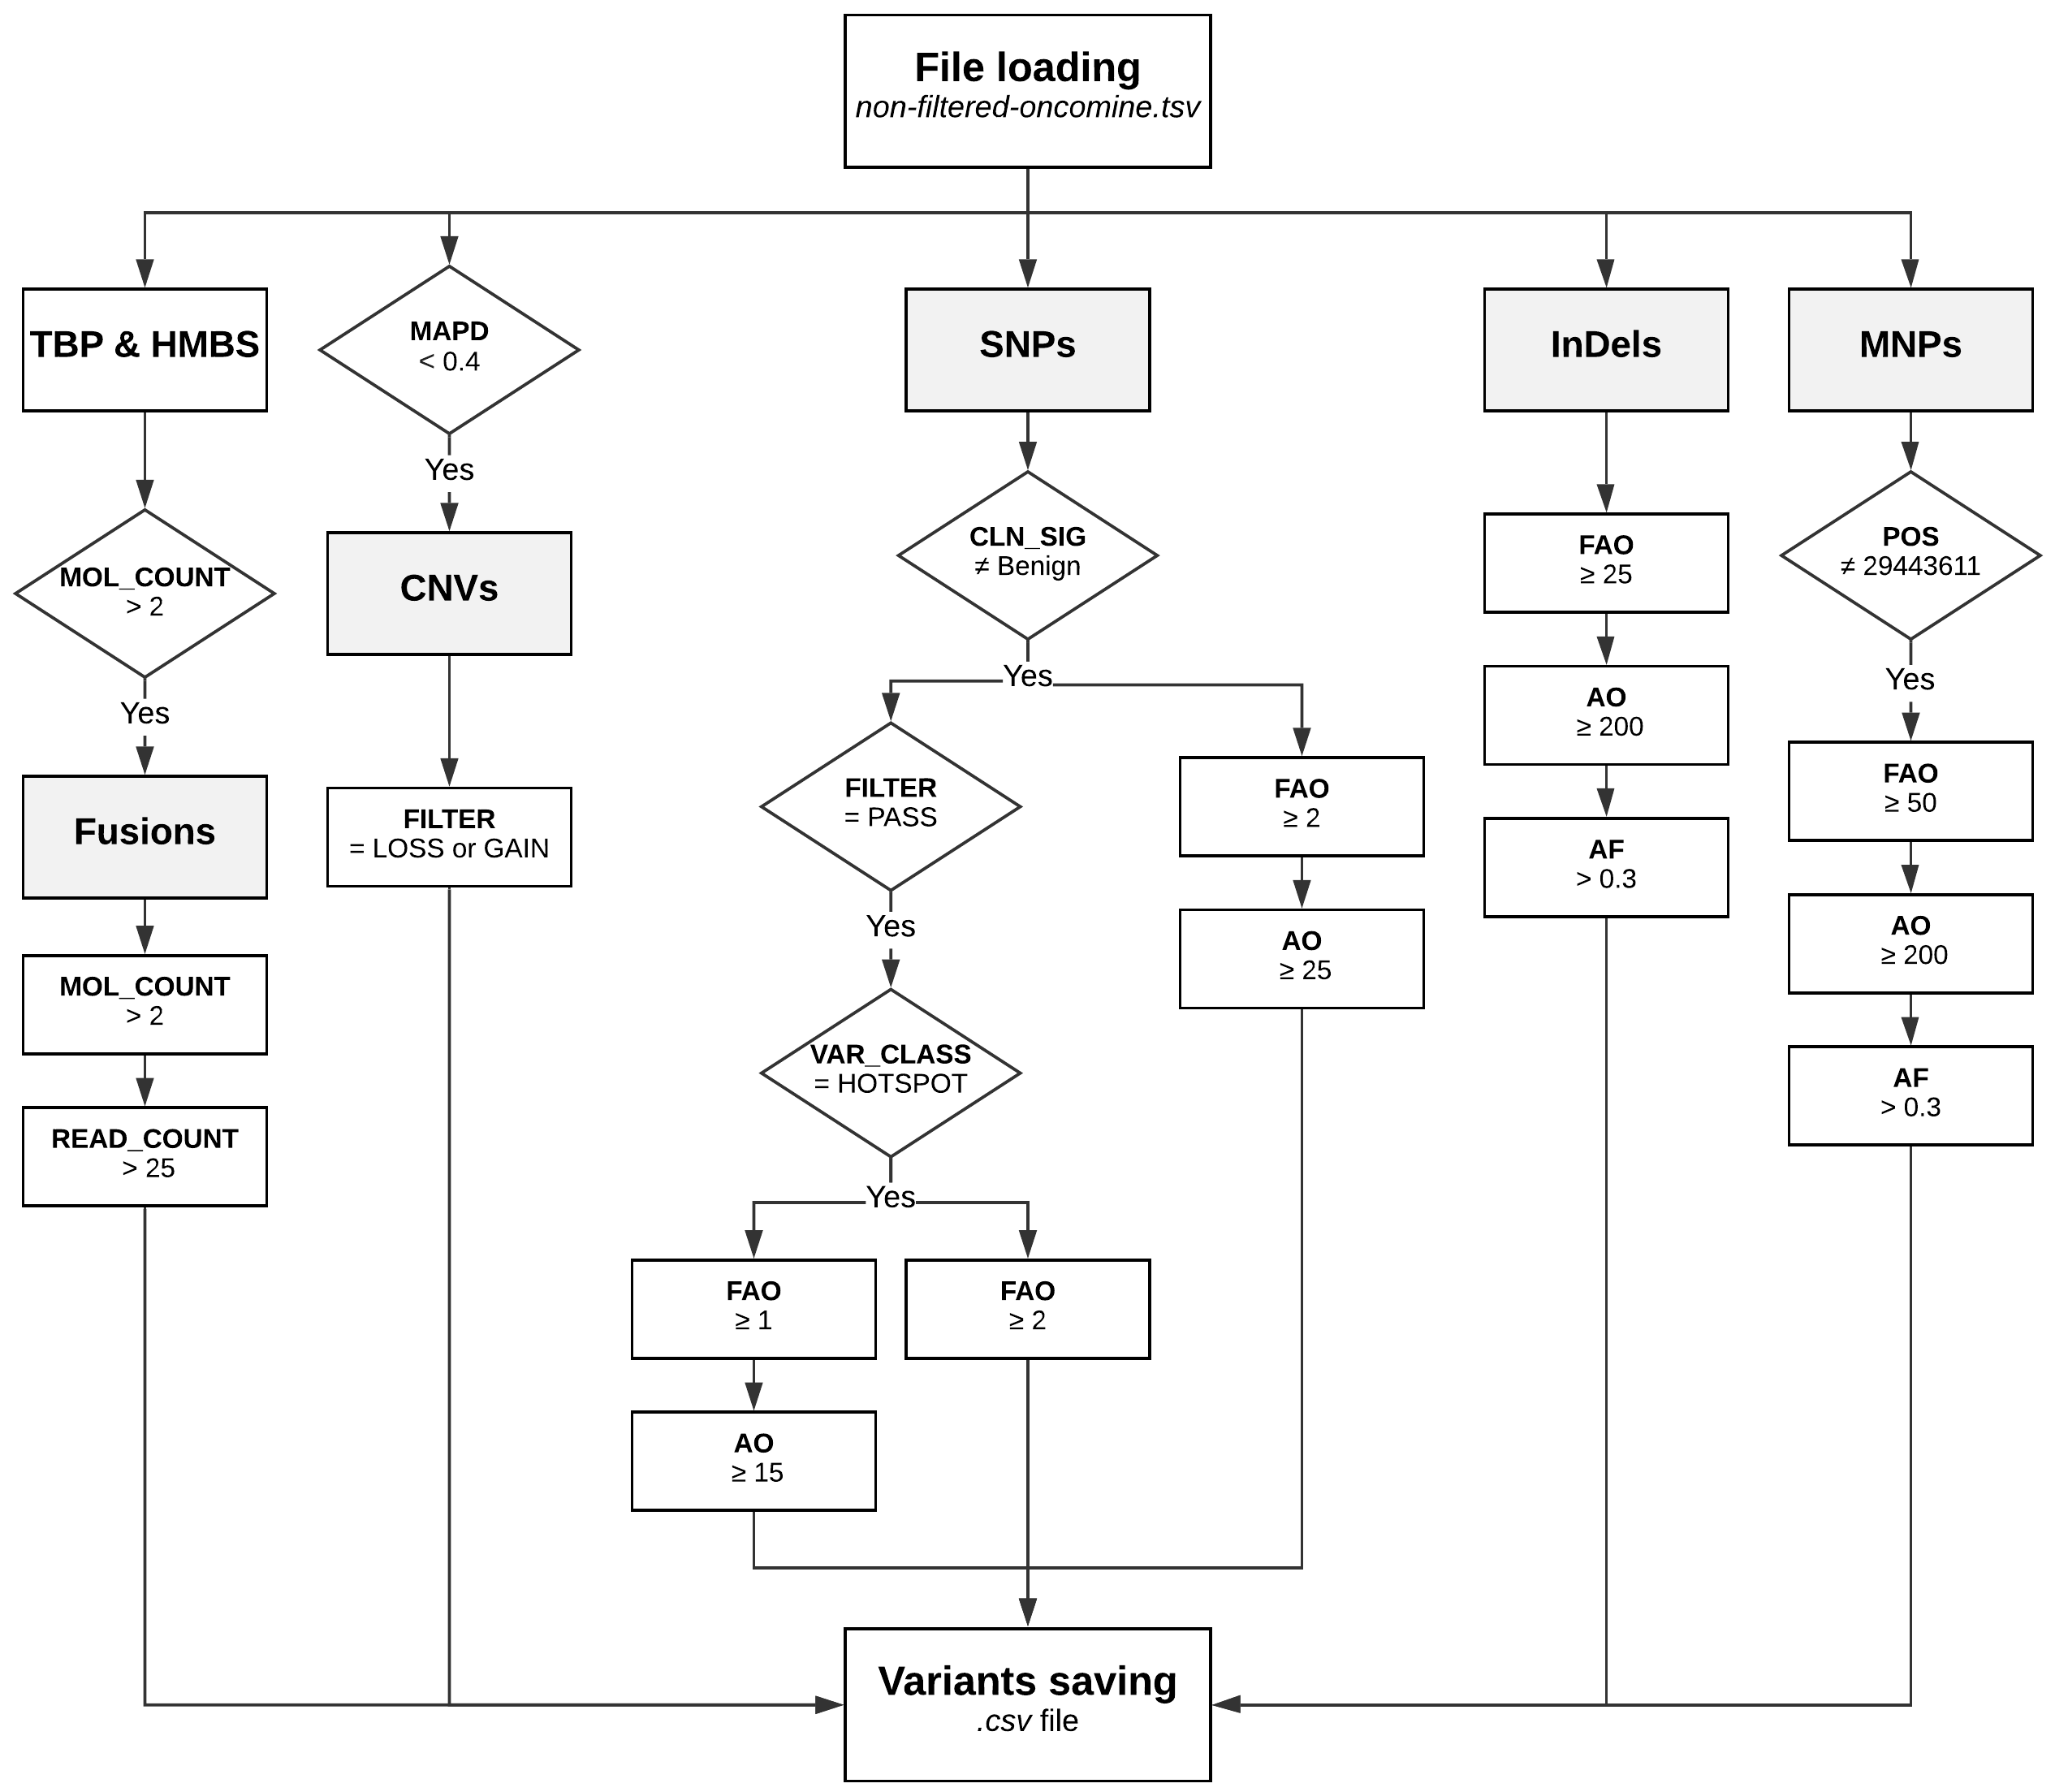
\includegraphics[width=\textwidth]{Images/chapter_4/mut_filtering.png}
    \caption{Flowchart of the bioinformatic pipeline optimized for the processing and assessment of variants at the ALK gene locus. MOL\_COUNT, molecular coverage; READ\_COUNT, read coverage; MAPD, median of the absolute values of all pairwise differences; FILTER: Ion Reporter\texttrademark{} internal filter (Oncomine\texttrademark{} Variants v5.12); CLN\_SIG, clinical significance; VAR\_CLASS: Oncomine\texttrademark{} Variant Class; POS: variant position; AF, allele frequency.}
    \label{fig:Algorithm}
\end{figure}

\subsubsection{Fusions Filtering}

The fusions filter selects translocations at the ALK locus with molecular coverage $> 2$, and fusion reads $> 25$. These thresholds have been established according to the clinical study data and the Oncomine\texttrademark{} Pan‐Cancer Cell‐Free Assay recommendations.

Additionally, two control genes were included in each sequencing process to measure the transcript abundance, TATA-binding protein (TBP) and hydroxymethylbilane synthase (HMBS). Both must have molecular coverage $> 2$ to validate the filtered fusion variants by ensuring their correct amplification.

\subsubsection{Copy-Number Variations Filtering}

Following the Ion Reporter\texttrademark{} recommendations, to make a CNV call the median of the absolute values of all pairwise differences (MAPD) must be $< 0.4$. MAPD measures the absolute difference between the $log_2$ copy-number ratios of adjacent amplicons and then calculates the median across all wells (\autoref{eq:MAPD}).
\begin{align} \label{eq:MAPD}
    MAPD &= median(\mid x_{i+1}-x_i \mid) \\
    \text{where}~
    x_i &\equiv \text{$log_2$ ratio for marker i} \notag
\end{align}

Larger MAPD values indicate lower coverage uniformity and greater noise, resulting in a higher probability of erroneous CNV calls. Therefore, only samples showing an MAPD $< 0.4$ were considered in further analysis, which consisted of selecting ALK gene copy-number gains or losses.

\subsubsection{Single-Nucleotide Polymorphisms Filtering}

Taking into account that false positives of this type of variants are not common, the proposed algorithm makes a call as long as any of the following conditions is met, discarding variants with a benign or likely benign clinical significance:
\begin{itemize}
    \item SNPs in hotspot regions that have passed the Oncomine\texttrademark{} Variants v5.12 filter and that have been detected in at least 1 molecular count with $\ge 15$ reads.
    \item SNPs in hotspot regions that have passed the Oncomine\texttrademark{} Variants v5.12 filter and that have been detected in at least 2 molecular counts.
    \item SNPs that have been detected in at least 2 molecular counts with $\ge 25$ reads.
\end{itemize}

\subsubsection{Insertions and Deletions Filtering}

The sequencing results usually present doubtful data regarding InDels. Therefore, the restrictions are more severe for this filter, which selects only variants that have been detected in at least 25 molecular counts with $\ge 200$ reads and an allele frequency (AF) $\ge 0.03$.

\subsubsection{Multiple-Nucleotide Polymorphisms Filtering}

Based on data from confirmed ALK-positive samples, false positives are highly likely in MNPs. In this context, only variants that have been detected in at least 50 molecular counts with $\ge 200$ reads and an AF $\ge 0.03$ were considered for confirmation by dPCR. 

On the other hand, abnormal Ion GeneStudio\texttrademark{} S5 Sequencer behavior at position chr2:29443611 of the ALK locus and involving the reading of 6 consecutive guanines (G) has been observed. Thus, variants at that location were excluded from further analysis.

\subsection{Graphical User Interface (GUI)}

The implemented user interface has been developed to facilitate data input and interpretation of results. The different layouts are shown in \autoref{fig:GUI}.

\begin{figure}[ht]
    \centering
    \begin{subfigure}{\textwidth}
        \centering
        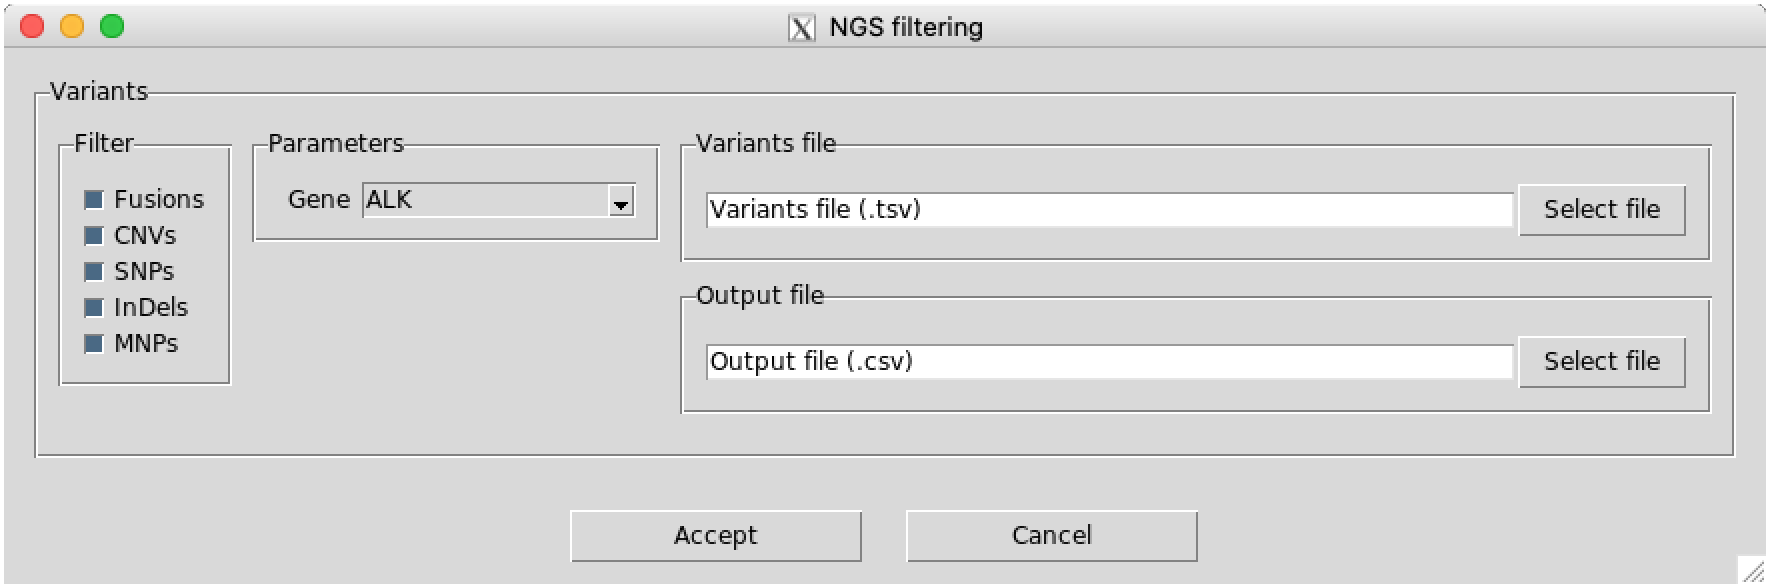
\includegraphics[width=\textwidth]{Images/chapter_4/GUI_1.png}
        \caption{Start screen. It allows selecting the type of variant\slash s to filter, the gene involved (ALK currently), as well as the source and output files. \\}
        \label{fig:GUI_1}
    \end{subfigure}
    \hfill
    \begin{subfigure}{0.47\textwidth}
        \centering
        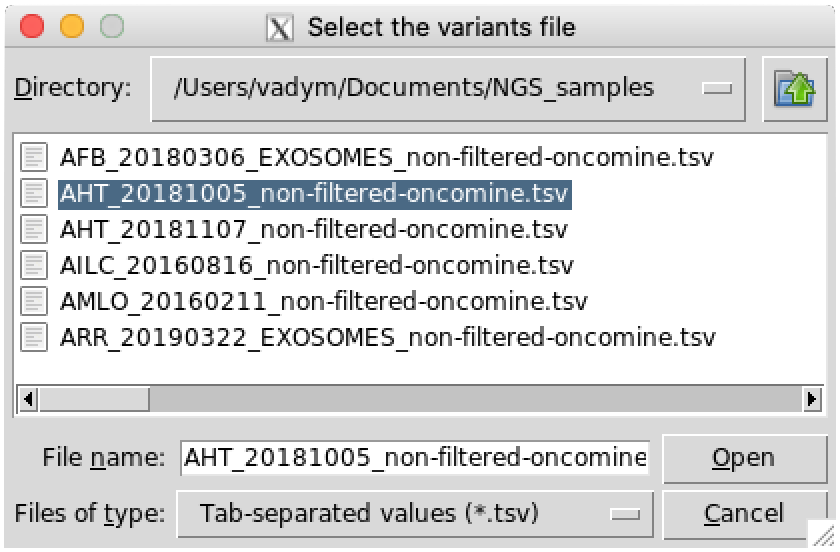
\includegraphics[width=\textwidth]{Images/chapter_4/GUI_2.png}
        \caption{Pop-up window for selecting the \textit{.tsv} source file containing raw variants.}
        \label{fig:GUI_2}
    \end{subfigure}
    \hfill
    \hfill
    \begin{subfigure}{0.52\textwidth}
        \centering
        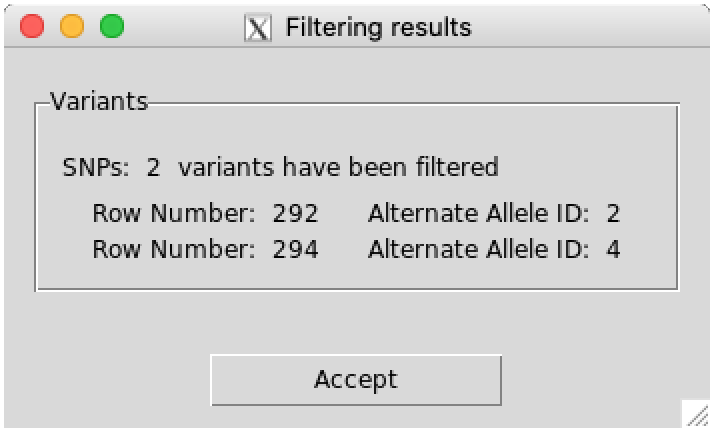
\includegraphics[width=\textwidth]{Images/chapter_4/GUI_3.png}
        \caption{Results screen showing 2 filtered SNPs, their $.tsv$ row number, and their alternate allele ID.}
        \label{fig:GUI_3}
    \end{subfigure}
    \hfill
    \caption{Implemented GUI showing the different display areas that appear throughout the filtering process.}
    \label{fig:GUI}
\end{figure}

The start screen (\autoref{fig:GUI_1}) has several options that allow some variability when proceeding with the filtering process. On the one hand, it is possible to select the filter\slash s to apply to the \textit{non-filtered-oncomine.tsv} file, as well as the gene to study. Currently, and as previously described, only the ALK gene has been addressed. On the other hand, the user can select both the source and output files through a pop-up screen, which is shown in \autoref{fig:GUI_2}. In case the output file does not exist, the program creates it automatically.

Finally, to fully characterize the variants that have passed a particular filter, the results are displayed specifying the mutation type, the row number of the variants in the \textit{non-filtered-oncomine.tsv} file, and the identifier of the alternate allele (\autoref{fig:GUI_3}). Simultaneously, each of the identified variants is appended to the $.csv$ output file along with its main characteristics.

It should also be noted that several additional screens have been implemented to offer the end-user information on the progress of the filtering process, on any errors that may have occurred during it, and on the non-identification of any variant of interest by the algorithm.

\section{Spectrum and Significance of Mutations}




% NSCLC_alterations
% Furthermore, tumours bearing co-mutations in TP53 exhibit higher degrees of copy number genomic instabi- lity (aneuploidy) and a higher somatic mutation burden, both on the trunk and in the branches of the tumour phylogenetic tree104. Therefore, TP53 co-mutations impact the natural history of EGFR-mutant NSCLC at least partially by allowing tolerance of a greater degree of genomic instability, which results in both larger num- bers of co-occurring truncal drivers and late subclonal diversification with focal emergence of high-amplitude amplifications and deletions in mediators of therapeutic resistance104. In keeping with a more complex genomic landscape and a larger burden of clonal or subclonal co-drivers, multiple clinical studies have identified TP53 co-alterations as a negative prognostic marker in EGFR-mutant LUAD and a consistent predictor of worse clinical outcomes following EGFR TKI therapy

% https://www.ncbi.nlm.nih.gov/pmc/articles/PMC6225899/
% In ALK-rearranged NSCLC co-occurring TP53 mutations predict an unfavorable outcome of systemic therapy.



\section{Statistic Analysis}

% Análisis estadístico
% Los resultados de frecuencia se expresarán en términos absolutos, en porcentajes e intervalos de confianza y, las variables cuantitativas como media ± desviación estándar o mediana (rango) según proceda.
% Para evaluar la concordancia del status de la translocación (positivo/negativo) entre las muestras de sangre (plaquetas y plasma) pre-tratamiento y el tejido se empleará el coeficiente Kappa de Cohen y su intervalo de confianza. Además, se analizará la sensibilidad, especificidad, valor predictivo positivo y valor predictivo negativo de la detección de la translocación en plasma (exosomas) y plaquetas, tomando como gold standar el resultado del tejido.
% Para analizar los datos de supervivencia de los pacientes se tomará como fecha de inicio, la fecha de inicio al tratamiento en primera línea y se recabarán los datos de: fecha de progresión, de muerte o fecha de última visita al oncólogo. La supervivencia libre de progresión se calculará desde la fecha de inicio al tratamiento en primera línea. Para el análisis de PFS y SG se usará el método de Kaplan-Meier y como estadístico de contraste se usará el Log- Rank. Los valores de los HR obtenidos serán ajustados por las variables clínico-patologícas pertinentes.
%Las pruebas con un valor de p <0.05 serán consideradas estadísticamente significativas.

\section{Utility}

% A key benefit for physicians is the serial use of digital PCR to monitor one or more driver mutations throughout treatment to determine response and recurrence since the level of mutated DNA found in liquid biopsies has been found to reflect the size of the tumor(s). It is also possible to use NGS to track progress; however, in these cases it is less practical due to cost and longer turnaround time.